% Options for packages loaded elsewhere
\PassOptionsToPackage{unicode}{hyperref}
\PassOptionsToPackage{hyphens}{url}
%
\documentclass[
]{article}
\usepackage{lmodern}
\usepackage{amssymb,amsmath}
\usepackage{ifxetex,ifluatex}
\ifnum 0\ifxetex 1\fi\ifluatex 1\fi=0 % if pdftex
  \usepackage[T1]{fontenc}
  \usepackage[utf8]{inputenc}
  \usepackage{textcomp} % provide euro and other symbols
\else % if luatex or xetex
  \usepackage{unicode-math}
  \defaultfontfeatures{Scale=MatchLowercase}
  \defaultfontfeatures[\rmfamily]{Ligatures=TeX,Scale=1}
\fi
% Use upquote if available, for straight quotes in verbatim environments
\IfFileExists{upquote.sty}{\usepackage{upquote}}{}
\IfFileExists{microtype.sty}{% use microtype if available
  \usepackage[]{microtype}
  \UseMicrotypeSet[protrusion]{basicmath} % disable protrusion for tt fonts
}{}
\makeatletter
\@ifundefined{KOMAClassName}{% if non-KOMA class
  \IfFileExists{parskip.sty}{%
    \usepackage{parskip}
  }{% else
    \setlength{\parindent}{0pt}
    \setlength{\parskip}{6pt plus 2pt minus 1pt}}
}{% if KOMA class
  \KOMAoptions{parskip=half}}
\makeatother
\usepackage{xcolor}
\IfFileExists{xurl.sty}{\usepackage{xurl}}{} % add URL line breaks if available
\IfFileExists{bookmark.sty}{\usepackage{bookmark}}{\usepackage{hyperref}}
\hypersetup{
  pdftitle={Simple 3-state microsimulation model with PSA},
  pdfauthor={The DARTH workgroup},
  hidelinks,
  pdfcreator={LaTeX via pandoc}}
\urlstyle{same} % disable monospaced font for URLs
\usepackage[margin=1in]{geometry}
\usepackage{color}
\usepackage{fancyvrb}
\newcommand{\VerbBar}{|}
\newcommand{\VERB}{\Verb[commandchars=\\\{\}]}
\DefineVerbatimEnvironment{Highlighting}{Verbatim}{commandchars=\\\{\}}
% Add ',fontsize=\small' for more characters per line
\usepackage{framed}
\definecolor{shadecolor}{RGB}{248,248,248}
\newenvironment{Shaded}{\begin{snugshade}}{\end{snugshade}}
\newcommand{\AlertTok}[1]{\textcolor[rgb]{0.94,0.16,0.16}{#1}}
\newcommand{\AnnotationTok}[1]{\textcolor[rgb]{0.56,0.35,0.01}{\textbf{\textit{#1}}}}
\newcommand{\AttributeTok}[1]{\textcolor[rgb]{0.77,0.63,0.00}{#1}}
\newcommand{\BaseNTok}[1]{\textcolor[rgb]{0.00,0.00,0.81}{#1}}
\newcommand{\BuiltInTok}[1]{#1}
\newcommand{\CharTok}[1]{\textcolor[rgb]{0.31,0.60,0.02}{#1}}
\newcommand{\CommentTok}[1]{\textcolor[rgb]{0.56,0.35,0.01}{\textit{#1}}}
\newcommand{\CommentVarTok}[1]{\textcolor[rgb]{0.56,0.35,0.01}{\textbf{\textit{#1}}}}
\newcommand{\ConstantTok}[1]{\textcolor[rgb]{0.00,0.00,0.00}{#1}}
\newcommand{\ControlFlowTok}[1]{\textcolor[rgb]{0.13,0.29,0.53}{\textbf{#1}}}
\newcommand{\DataTypeTok}[1]{\textcolor[rgb]{0.13,0.29,0.53}{#1}}
\newcommand{\DecValTok}[1]{\textcolor[rgb]{0.00,0.00,0.81}{#1}}
\newcommand{\DocumentationTok}[1]{\textcolor[rgb]{0.56,0.35,0.01}{\textbf{\textit{#1}}}}
\newcommand{\ErrorTok}[1]{\textcolor[rgb]{0.64,0.00,0.00}{\textbf{#1}}}
\newcommand{\ExtensionTok}[1]{#1}
\newcommand{\FloatTok}[1]{\textcolor[rgb]{0.00,0.00,0.81}{#1}}
\newcommand{\FunctionTok}[1]{\textcolor[rgb]{0.00,0.00,0.00}{#1}}
\newcommand{\ImportTok}[1]{#1}
\newcommand{\InformationTok}[1]{\textcolor[rgb]{0.56,0.35,0.01}{\textbf{\textit{#1}}}}
\newcommand{\KeywordTok}[1]{\textcolor[rgb]{0.13,0.29,0.53}{\textbf{#1}}}
\newcommand{\NormalTok}[1]{#1}
\newcommand{\OperatorTok}[1]{\textcolor[rgb]{0.81,0.36,0.00}{\textbf{#1}}}
\newcommand{\OtherTok}[1]{\textcolor[rgb]{0.56,0.35,0.01}{#1}}
\newcommand{\PreprocessorTok}[1]{\textcolor[rgb]{0.56,0.35,0.01}{\textit{#1}}}
\newcommand{\RegionMarkerTok}[1]{#1}
\newcommand{\SpecialCharTok}[1]{\textcolor[rgb]{0.00,0.00,0.00}{#1}}
\newcommand{\SpecialStringTok}[1]{\textcolor[rgb]{0.31,0.60,0.02}{#1}}
\newcommand{\StringTok}[1]{\textcolor[rgb]{0.31,0.60,0.02}{#1}}
\newcommand{\VariableTok}[1]{\textcolor[rgb]{0.00,0.00,0.00}{#1}}
\newcommand{\VerbatimStringTok}[1]{\textcolor[rgb]{0.31,0.60,0.02}{#1}}
\newcommand{\WarningTok}[1]{\textcolor[rgb]{0.56,0.35,0.01}{\textbf{\textit{#1}}}}
\usepackage{graphicx,grffile}
\makeatletter
\def\maxwidth{\ifdim\Gin@nat@width>\linewidth\linewidth\else\Gin@nat@width\fi}
\def\maxheight{\ifdim\Gin@nat@height>\textheight\textheight\else\Gin@nat@height\fi}
\makeatother
% Scale images if necessary, so that they will not overflow the page
% margins by default, and it is still possible to overwrite the defaults
% using explicit options in \includegraphics[width, height, ...]{}
\setkeys{Gin}{width=\maxwidth,height=\maxheight,keepaspectratio}
% Set default figure placement to htbp
\makeatletter
\def\fps@figure{htbp}
\makeatother
\setlength{\emergencystretch}{3em} % prevent overfull lines
\providecommand{\tightlist}{%
  \setlength{\itemsep}{0pt}\setlength{\parskip}{0pt}}
\setcounter{secnumdepth}{-\maxdimen} % remove section numbering

\title{Simple 3-state microsimulation model with PSA}
\usepackage{etoolbox}
\makeatletter
\providecommand{\subtitle}[1]{% add subtitle to \maketitle
  \apptocmd{\@title}{\par {\large #1 \par}}{}{}
}
\makeatother
\subtitle{Includes sex specific probability of dying when healthy and state
occupation: probability of dying when sick depends on the time of being
sick}
\author{The DARTH workgroup}
\date{}

\begin{document}
\maketitle

Developed by the Decision Analysis in R for Technologies in Health
(DARTH) workgroup:

Fernando Alarid-Escudero, PhD (1)

Eva A. Enns, MS, PhD (2)

M.G. Myriam Hunink, MD, PhD (3,4)

Hawre J. Jalal, MD, PhD (5)

Eline M. Krijkamp, MSc (3)

Petros Pechlivanoglou, PhD (6,7)

Alan Yang, MSc (7)

In collaboration of:

\begin{enumerate}
\def\labelenumi{\arabic{enumi}.}
\tightlist
\item
  Drug Policy Program, Center for Research and Teaching in Economics
  (CIDE) - CONACyT, Aguascalientes, Mexico
\item
  University of Minnesota School of Public Health, Minneapolis, MN, USA
\item
  Erasmus MC, Rotterdam, The Netherlands
\item
  Harvard T.H. Chan School of Public Health, Boston, USA
\item
  University of Pittsburgh Graduate School of Public Health, Pittsburgh,
  PA, USA
\item
  University of Toronto, Toronto ON, Canada
\item
  The Hospital for Sick Children, Toronto ON, Canada
\end{enumerate}

Please cite our publications when using this code:

\begin{itemize}
\item
  Jalal H, Pechlivanoglou P, Krijkamp E, Alarid-Escudero F, Enns E,
  Hunink MG. An Overview of R in Health Decision Sciences. Med Decis
  Making. 2017; 37(3): 735-746.
  \url{https://journals.sagepub.com/doi/abs/10.1177/0272989X16686559}
\item
  Krijkamp EM, Alarid-Escudero F, Enns EA, Jalal HJ, Hunink MGM,
  Pechlivanoglou P. Microsimulation modeling for health decision
  sciences using R: A tutorial. Med Decis Making. 2018;38(3):400--22.
  \url{https://journals.sagepub.com/doi/abs/10.1177/0272989X18754513}
\item
  Krijkamp EM, Alarid-Escudero F, Enns E, Pechlivanoglou P, Hunink MM,
  Jalal H. A Multidimensional Array Representation of State-Transition
  Model Dynamics. Med Decis Making. 2020 Online first.
  \url{https://doi.org/10.1177/0272989X19893973}
\end{itemize}

Copyright 2017, THE HOSPITAL FOR SICK CHILDREN AND THE COLLABORATING
INSTITUTIONS. All rights reserved in Canada, the United States and
worldwide. Copyright, trademarks, trade names and any and all associated
intellectual property are exclusively owned by THE HOSPITAL FOR Sick
CHILDREN and the collaborating institutions. These materials may be
used, reproduced, modified, distributed and adapted with proper
attribution.

\newpage

\begin{Shaded}
\begin{Highlighting}[]
\KeywordTok{rm}\NormalTok{(}\DataTypeTok{list =} \KeywordTok{ls}\NormalTok{())      }\CommentTok{# clear memory (removes all the variables from the workspace)}
\end{Highlighting}
\end{Shaded}

\hypertarget{load-packages}{%
\section{01 Load packages}\label{load-packages}}

\begin{Shaded}
\begin{Highlighting}[]
\ControlFlowTok{if}\NormalTok{ (}\OperatorTok{!}\KeywordTok{require}\NormalTok{(}\StringTok{'pacman'}\NormalTok{)) }\KeywordTok{install.packages}\NormalTok{(}\StringTok{'pacman'}\NormalTok{); }\KeywordTok{library}\NormalTok{(pacman) }\CommentTok{# use this package to conveniently install other packages}
 \CommentTok{# load (install if required) packages from CRAN}
 \KeywordTok{p_load}\NormalTok{(}\StringTok{"here"}\NormalTok{, }\StringTok{"dplyr"}\NormalTok{, }\StringTok{"devtools"}\NormalTok{, }\StringTok{"scales"}\NormalTok{, }\StringTok{"ellipse"}\NormalTok{, }\StringTok{"ggplot2"}\NormalTok{, }\StringTok{"lazyeval"}\NormalTok{, }\StringTok{"igraph"}\NormalTok{, }\StringTok{"ggraph"}\NormalTok{, }\StringTok{"reshape2"}\NormalTok{, }\StringTok{"knitr"}\NormalTok{)                                               }
 \CommentTok{# load (install if required) packages from GitHub}
 \CommentTok{# install_github("DARTH-git/dampack", force = TRUE) Uncomment if there is a newer version}
 \KeywordTok{p_load_gh}\NormalTok{(}\StringTok{"DARTH-git/dampack"}\NormalTok{) }
\end{Highlighting}
\end{Shaded}

\hypertarget{load-functions}{%
\section{02 Load functions}\label{load-functions}}

\begin{Shaded}
\begin{Highlighting}[]
\KeywordTok{source}\NormalTok{(}\StringTok{"Functions.R"}\NormalTok{)  }\CommentTok{# This line only works when you "Function.R" file is in the same folder}
\end{Highlighting}
\end{Shaded}

\hypertarget{input-model-parameters}{%
\section{03 Input model parameters}\label{input-model-parameters}}

\begin{Shaded}
\begin{Highlighting}[]
\KeywordTok{set.seed}\NormalTok{(}\DecValTok{1}\NormalTok{)  }\CommentTok{# set the seed  }

\CommentTok{# Model structure}
\NormalTok{v_n   <-}\StringTok{ }\KeywordTok{c}\NormalTok{(}\StringTok{"healthy"}\NormalTok{, }\StringTok{"sick"}\NormalTok{, }\StringTok{"dead"}\NormalTok{)          }\CommentTok{# vector with state names}
\NormalTok{n_states   <-}\StringTok{ }\KeywordTok{length}\NormalTok{(v_n)                      }\CommentTok{# number of states}
\NormalTok{n_t   <-}\StringTok{ }\DecValTok{60}                                    \CommentTok{# number of cycles}
\NormalTok{n_i   <-}\StringTok{ }\DecValTok{10000}                                 \CommentTok{# number of individuals}
\NormalTok{d_e <-}\StringTok{ }\NormalTok{d_c <-}\StringTok{ }\FloatTok{0.03}                             \CommentTok{# equal discount of costs and QALYs by 3%}

\CommentTok{# calculate discount weights for costs for each cycle based on discount rate d_c}
\NormalTok{v_dwc <-}\StringTok{ }\DecValTok{1} \OperatorTok{/}\StringTok{ }\NormalTok{(}\DecValTok{1} \OperatorTok{+}\StringTok{ }\NormalTok{d_e) }\OperatorTok{^}\StringTok{ }\NormalTok{(}\DecValTok{0}\OperatorTok{:}\NormalTok{n_t) }
\CommentTok{# calculate discount weights for effectiveness for each cycle based on discount rate d_e}
\NormalTok{v_dwe <-}\StringTok{ }\DecValTok{1} \OperatorTok{/}\StringTok{ }\NormalTok{(}\DecValTok{1} \OperatorTok{+}\StringTok{ }\NormalTok{d_c) }\OperatorTok{^}\StringTok{ }\NormalTok{(}\DecValTok{0}\OperatorTok{:}\NormalTok{n_t) }

\CommentTok{#### Deterministic analysis ####}

\CommentTok{# Transition probabilities}
\NormalTok{p_HS <-}\StringTok{ }\FloatTok{0.05}           \CommentTok{# probability healthy -> sick}
\NormalTok{p_HD_female <-}\StringTok{ }\FloatTok{0.0382}  \CommentTok{# probability health -> dead when female}
\NormalTok{p_HD_male   <-}\StringTok{ }\FloatTok{0.0463}  \CommentTok{# probability health -> dead when male}
\NormalTok{m_p_HD      <-}\StringTok{ }\KeywordTok{data.frame}\NormalTok{(}\DataTypeTok{Sex =} \KeywordTok{c}\NormalTok{(}\StringTok{"Female"}\NormalTok{, }\StringTok{"Male"}\NormalTok{), }\DataTypeTok{p_HD =} \KeywordTok{c}\NormalTok{(p_HD_female, p_HD_male)) }\CommentTok{# combine the probabilities in a dataframe }

\CommentTok{# probability to die in sick state by cycle of being sick}
\NormalTok{p_SD <-}\StringTok{ }\KeywordTok{c}\NormalTok{(}\FloatTok{0.1}\NormalTok{, }\FloatTok{0.2}\NormalTok{, }\FloatTok{0.3}\NormalTok{, }\FloatTok{0.4}\NormalTok{, }\FloatTok{0.5}\NormalTok{, }\KeywordTok{rep}\NormalTok{(}\FloatTok{0.7}\NormalTok{, n_t }\OperatorTok{-}\StringTok{ }\DecValTok{5}\NormalTok{)) }

\CommentTok{# Costs inputs}
\NormalTok{c_H  <-}\StringTok{ }\DecValTok{1500}      \CommentTok{# cost of one cycle in healthy state}
\NormalTok{c_S  <-}\StringTok{ }\DecValTok{5000}      \CommentTok{# cost of one cycle in sick state}
\NormalTok{c_D  <-}\StringTok{ }\DecValTok{0}

\CommentTok{# utility inputs}
\NormalTok{u_H  <-}\StringTok{ }\DecValTok{1}         \CommentTok{# utility when healthy }
\NormalTok{u_S  <-}\StringTok{ }\FloatTok{0.85}      \CommentTok{# utility when sick }
\NormalTok{u_D  <-}\StringTok{ }\DecValTok{0}         \CommentTok{# utility when dead }
\end{Highlighting}
\end{Shaded}

\hypertarget{sample-individual-level-characteristics}{%
\section{04 Sample individual level
characteristics}\label{sample-individual-level-characteristics}}

\hypertarget{static-characteristics}{%
\subsection{04.1 Static characteristics}\label{static-characteristics}}

\begin{Shaded}
\begin{Highlighting}[]
\CommentTok{# randomly sample the sex of an individual (50% female)}
\NormalTok{v_sex <-}\StringTok{ }\KeywordTok{sample}\NormalTok{(}\DataTypeTok{x =} \KeywordTok{c}\NormalTok{(}\StringTok{"Female"}\NormalTok{, }\StringTok{"Male"}\NormalTok{), }\DataTypeTok{prob =} \KeywordTok{c}\NormalTok{(}\FloatTok{0.5}\NormalTok{, }\FloatTok{0.5}\NormalTok{), }\DataTypeTok{size =}\NormalTok{ n_i, }\DataTypeTok{replace =} \OtherTok{TRUE}\NormalTok{) }
\NormalTok{df_X  <-}\StringTok{ }\KeywordTok{data.frame}\NormalTok{(}\DataTypeTok{ID =} \DecValTok{1}\OperatorTok{:}\NormalTok{n_i, }\DataTypeTok{Sex =}\NormalTok{ v_sex) }\CommentTok{# Make a data frame of the individual cahracteristics}
\end{Highlighting}
\end{Shaded}

\hypertarget{dynamic-characteristics}{%
\subsection{04.2 Dynamic
characteristics}\label{dynamic-characteristics}}

\begin{Shaded}
\begin{Highlighting}[]
\CommentTok{# Specify the initial health state of the individuals }
\CommentTok{# everyone begins in the healthy state (in this example)}
\NormalTok{v_M_init  <-}\StringTok{ }\KeywordTok{rep}\NormalTok{(}\StringTok{"healthy"}\NormalTok{, }\DataTypeTok{times =}\NormalTok{ n_i)   }
\NormalTok{v_Ts_init <-}\StringTok{ }\KeywordTok{rep}\NormalTok{(}\DecValTok{0}\NormalTok{, n_i)  }\CommentTok{# a vector with the time of being sick at the start of the model }
\end{Highlighting}
\end{Shaded}

\hypertarget{define-simulation-functions}{%
\section{05 Define Simulation
Functions}\label{define-simulation-functions}}

\hypertarget{probability-function}{%
\subsection{05.1 Probability function}\label{probability-function}}

The function that updates the transition probabilities of every cycle is
shown below.

\begin{Shaded}
\begin{Highlighting}[]
\NormalTok{Probs <-}\StringTok{ }\ControlFlowTok{function}\NormalTok{(M_t, df_X, v_Ts) \{ }
  \CommentTok{# Arguments:}
    \CommentTok{# M_t: health state occupied at cycle t (character variable)}
    \CommentTok{# df_X: data frame with individual characteristics data }
    \CommentTok{# v_Ts: vector with the duration of being sick}
  \CommentTok{# Returns: }
    \CommentTok{# transition probabilities for that cycle}
  
  \CommentTok{# create matrix of state transition probabilities}
\NormalTok{  m_p_t           <-}\StringTok{ }\KeywordTok{matrix}\NormalTok{(}\DecValTok{0}\NormalTok{, }\DataTypeTok{nrow =}\NormalTok{ n_states, }\DataTypeTok{ncol =}\NormalTok{ n_i)  }
  \CommentTok{# give the state names to the rows}
  \KeywordTok{rownames}\NormalTok{(m_p_t) <-}\StringTok{  }\NormalTok{v_n                               }
  
  \CommentTok{# lookup baseline probability and rate of dying based on individual characteristics}
\NormalTok{  p_HD_all <-}\StringTok{ }\KeywordTok{inner_join}\NormalTok{(df_X, m_p_HD, }\DataTypeTok{by =} \KeywordTok{c}\NormalTok{(}\StringTok{"Sex"}\NormalTok{) )}
\NormalTok{  p_HD     <-}\StringTok{ }\NormalTok{p_HD_all[M_t }\OperatorTok{==}\StringTok{ "healthy"}\NormalTok{, }\StringTok{"p_HD"}\NormalTok{]}
  
  \CommentTok{# update m_p_t with the appropriate probabilities   }
  \CommentTok{# transition probabilities when healthy}
\NormalTok{  m_p_t[, M_t }\OperatorTok{==}\StringTok{ "healthy"}\NormalTok{] <-}\StringTok{ }\KeywordTok{rbind}\NormalTok{(}\DecValTok{1} \OperatorTok{-}\StringTok{ }\NormalTok{p_HD }\OperatorTok{-}\StringTok{ }\NormalTok{p_HS, p_HS, p_HD)    }
  \CommentTok{# transition probabilities when sick }
\NormalTok{  m_p_t[, M_t }\OperatorTok{==}\StringTok{ "sick"}\NormalTok{]    <-}\StringTok{ }\KeywordTok{rbind}\NormalTok{(}\DecValTok{0}\NormalTok{, }\DecValTok{1} \OperatorTok{-}\StringTok{ }\NormalTok{p_SD[v_Ts], p_SD[v_Ts])  }
  \CommentTok{# transition probabilities when dead     }
\NormalTok{  m_p_t[, M_t }\OperatorTok{==}\StringTok{ "dead"}\NormalTok{]    <-}\StringTok{ }\KeywordTok{rbind}\NormalTok{(}\DecValTok{0}\NormalTok{, }\DecValTok{0}\NormalTok{, }\DecValTok{1}\NormalTok{)                            }
  \KeywordTok{return}\NormalTok{(}\KeywordTok{t}\NormalTok{(m_p_t))}
\NormalTok{\}       }
\end{Highlighting}
\end{Shaded}

\hypertarget{cost-function}{%
\subsection{05.2 Cost function}\label{cost-function}}

The \texttt{Costs} function estimates the costs at every cycle.

\begin{Shaded}
\begin{Highlighting}[]
\NormalTok{Costs <-}\StringTok{ }\ControlFlowTok{function}\NormalTok{ (M_t) \{}
  \CommentTok{# M_t: current health state}
\NormalTok{  c_t <-}\StringTok{ }\KeywordTok{c}\NormalTok{()}
\NormalTok{  c_t[M_t }\OperatorTok{==}\StringTok{ "dead"}\NormalTok{]    <-}\StringTok{ }\NormalTok{c_D     }\CommentTok{# costs at dead state}
\NormalTok{  c_t[M_t }\OperatorTok{==}\StringTok{ "healthy"}\NormalTok{] <-}\StringTok{ }\NormalTok{c_H     }\CommentTok{# costs accrued by being healthy this cycle}
\NormalTok{  c_t[M_t }\OperatorTok{==}\StringTok{ "sick"}\NormalTok{]    <-}\StringTok{ }\NormalTok{c_S     }\CommentTok{# costs accrued by being sick this cycle}
  
  \KeywordTok{return}\NormalTok{(c_t)  }\CommentTok{# return costs accrued this cycle}
\NormalTok{\}}
\end{Highlighting}
\end{Shaded}

\hypertarget{health-outcome-function}{%
\subsection{05.3 Health outcome
function}\label{health-outcome-function}}

The \texttt{Effs} function to update the utilities at every cycle.

\begin{Shaded}
\begin{Highlighting}[]
\NormalTok{Effs <-}\StringTok{ }\ControlFlowTok{function}\NormalTok{ (M_t) \{}
  \CommentTok{# M_t: current health state}
\NormalTok{  q_t <-}\StringTok{ }\KeywordTok{c}\NormalTok{() }
\NormalTok{  q_t[M_t }\OperatorTok{==}\StringTok{ "dead"}\NormalTok{]    <-}\StringTok{ }\NormalTok{u_D     }\CommentTok{# QALYs at dead state}
\NormalTok{  q_t[M_t }\OperatorTok{==}\StringTok{ "healthy"}\NormalTok{] <-}\StringTok{ }\NormalTok{u_H     }\CommentTok{# QALYs accrued by being healthy this cycle}
\NormalTok{  q_t[M_t }\OperatorTok{==}\StringTok{ "sick"}\NormalTok{]    <-}\StringTok{ }\NormalTok{u_S     }\CommentTok{# QALYs accrued by being sick this cycle}
  
  \KeywordTok{return}\NormalTok{(q_t)  }\CommentTok{# return the QALYs accrued this cycle}
\NormalTok{\}}
\end{Highlighting}
\end{Shaded}

\hypertarget{run-microsimulation}{%
\section{06 Run Microsimulation}\label{run-microsimulation}}

\begin{Shaded}
\begin{Highlighting}[]
\NormalTok{MicroSim <-}\StringTok{ }\ControlFlowTok{function}\NormalTok{(n_i, df_X, }\DataTypeTok{seed =} \DecValTok{1}\NormalTok{) \{}
  \CommentTok{# Arguments:  }
    \CommentTok{# n_i:     number of individuals}
    \CommentTok{# df_X     data frame with individual data }
    \CommentTok{# seed: default is 1}
  \CommentTok{# Returns:}
    \CommentTok{# results: a list if microsimulation results}
  
  \KeywordTok{set.seed}\NormalTok{(seed) }\CommentTok{# set the seed}
  
  \CommentTok{# create three matrices called m_M, m_C and m_E}
  \CommentTok{# number of rows is equal to the n_i, the number of columns is equal to n_t }
  \CommentTok{# (the initial state and all the n_t cycles)}
  \CommentTok{# m_M is used to store the health state information over time for every individual}
  \CommentTok{# m_C is used to store the costs information over time for every individual}
  \CommentTok{# m_E is used to store the effects information over time for every individual}
  
\NormalTok{  m_M <-}\StringTok{ }\NormalTok{m_C <-}\StringTok{ }\NormalTok{m_E <-}\StringTok{  }\KeywordTok{matrix}\NormalTok{(}\DataTypeTok{nrow =}\NormalTok{ n_i, }\DataTypeTok{ncol =}\NormalTok{ n_t }\OperatorTok{+}\StringTok{ }\DecValTok{1}\NormalTok{, }
                                       \DataTypeTok{dimnames =} \KeywordTok{list}\NormalTok{(}\KeywordTok{paste}\NormalTok{(}\StringTok{"ind"}\NormalTok{  , }\DecValTok{1}\OperatorTok{:}\NormalTok{n_i, }\DataTypeTok{sep =} \StringTok{" "}\NormalTok{), }
                                                       \KeywordTok{paste}\NormalTok{(}\StringTok{"cycle"}\NormalTok{, }\DecValTok{0}\OperatorTok{:}\NormalTok{n_t, }\DataTypeTok{sep =} \StringTok{" "}\NormalTok{)))  }
 
\NormalTok{  m_M[, }\DecValTok{1}\NormalTok{] <-}\StringTok{ }\NormalTok{v_M_init          }\CommentTok{# initial health state}
\NormalTok{  v_Ts     <-}\StringTok{ }\NormalTok{v_Ts_init         }\CommentTok{# initialize time since illnes onset}
\NormalTok{  m_C[, }\DecValTok{1}\NormalTok{] <-}\StringTok{ }\KeywordTok{Costs}\NormalTok{(m_M[, }\DecValTok{1}\NormalTok{])   }\CommentTok{# costs accrued during cycle 0}
\NormalTok{  m_E[, }\DecValTok{1}\NormalTok{] <-}\StringTok{ }\KeywordTok{Effs}\NormalTok{(m_M[, }\DecValTok{1}\NormalTok{])    }\CommentTok{# QALYs accrued during cycle 0}
  
  \CommentTok{# open a loop for time running cycles 1 to n_t }
  \ControlFlowTok{for}\NormalTok{ (t }\ControlFlowTok{in} \DecValTok{1}\OperatorTok{:}\NormalTok{n_t) \{}
    \CommentTok{# calculate the transition probabilities for the cycle based on health state t}
\NormalTok{    m_P <-}\StringTok{ }\KeywordTok{Probs}\NormalTok{(m_M[, t], df_X, v_Ts)  }
    \CommentTok{# sample the current health state and store that state in matrix m_M}
\NormalTok{    m_M[, t }\OperatorTok{+}\StringTok{ }\DecValTok{1}\NormalTok{]  <-}\StringTok{ }\KeywordTok{samplev}\NormalTok{(m_P, }\DecValTok{1}\NormalTok{)    }
    \CommentTok{# calculate costs per individual during cycle t + 1}
\NormalTok{    m_C[, t }\OperatorTok{+}\StringTok{ }\DecValTok{1}\NormalTok{]  <-}\StringTok{ }\KeywordTok{Costs}\NormalTok{(m_M[, t }\OperatorTok{+}\StringTok{ }\DecValTok{1}\NormalTok{])  }
    \CommentTok{# calculate QALYs per individual during cycle t + 1}
\NormalTok{    m_E[, t }\OperatorTok{+}\StringTok{ }\DecValTok{1}\NormalTok{]  <-}\StringTok{ }\KeywordTok{Effs}\NormalTok{ (m_M[, t }\OperatorTok{+}\StringTok{ }\DecValTok{1}\NormalTok{])  }
    
    \CommentTok{# update time since illness onset for t + 1 }
\NormalTok{    v_Ts <-}\StringTok{ }\KeywordTok{if_else}\NormalTok{(m_M[, t }\OperatorTok{+}\StringTok{ }\DecValTok{1}\NormalTok{] }\OperatorTok{==}\StringTok{ "sick"}\NormalTok{, v_Ts }\OperatorTok{+}\StringTok{ }\DecValTok{1}\NormalTok{, }\DecValTok{0}\NormalTok{) }
    
    \CommentTok{# Display simulation progress}
    \ControlFlowTok{if}\NormalTok{(t}\OperatorTok{/}\NormalTok{(n_t}\OperatorTok{/}\DecValTok{10}\NormalTok{) }\OperatorTok{==}\StringTok{ }\KeywordTok{round}\NormalTok{(t}\OperatorTok{/}\NormalTok{(n_t}\OperatorTok{/}\DecValTok{10}\NormalTok{), }\DecValTok{0}\NormalTok{)) \{ }\CommentTok{# display progress every 10%}
      \KeywordTok{cat}\NormalTok{(}\StringTok{'}\CharTok{\textbackslash{}r}\StringTok{'}\NormalTok{, }\KeywordTok{paste}\NormalTok{(t}\OperatorTok{/}\NormalTok{n_t }\OperatorTok{*}\StringTok{ }\DecValTok{100}\NormalTok{, }\StringTok{"% done"}\NormalTok{, }\DataTypeTok{sep =} \StringTok{" "}\NormalTok{))}
\NormalTok{    \}}
    
\NormalTok{  \} }\CommentTok{# close the loop for the time points }
  
  \CommentTok{# calculate  }
\NormalTok{  tc <-}\StringTok{ }\NormalTok{m_C }\OperatorTok\StringTok{ }\NormalTok{v_dwc    }\CommentTok{# total (discounted) cost per individual}
\NormalTok{  te <-}\StringTok{ }\NormalTok{m_E }\OperatorTok\StringTok{ }\NormalTok{v_dwe    }\CommentTok{# total (discounted) QALYs per individual }
\NormalTok{  tc_hat <-}\StringTok{ }\KeywordTok{mean}\NormalTok{(tc)     }\CommentTok{# average (discounted) cost }
\NormalTok{  te_hat <-}\StringTok{ }\KeywordTok{mean}\NormalTok{(te)     }\CommentTok{# average (discounted) QALYs}
  
  \CommentTok{# store the results from the simulation in a list}
\NormalTok{  results <-}\StringTok{ }\KeywordTok{list}\NormalTok{(}\DataTypeTok{m_M =}\NormalTok{ m_M, }\DataTypeTok{m_C =}\NormalTok{ m_C, }\DataTypeTok{m_E =}\NormalTok{ m_E, }\DataTypeTok{tc =}\NormalTok{ tc , }\DataTypeTok{te =}\NormalTok{ te, }\DataTypeTok{tc_hat =}\NormalTok{ tc_hat, }
                  \DataTypeTok{te_hat =}\NormalTok{ te_hat)   }
  
  \KeywordTok{return}\NormalTok{(results)  }\CommentTok{# return the results}

\NormalTok{\} }\CommentTok{# end of the MicroSim function  }

\CommentTok{# By specifying all the arguments in the `MicroSim()` the simulation can be started}

\CommentTok{# Run the simulation model}
\NormalTok{outcomes <-}\StringTok{ }\KeywordTok{MicroSim}\NormalTok{(n_i, df_X, }\DataTypeTok{seed =} \DecValTok{1}\NormalTok{)}
\end{Highlighting}
\end{Shaded}

\begin{verbatim}
##  10 % done 20 % done 30 % done 40 % done 50 % done 60 % done 70 % done 80 % done 90 % done 100 % done
\end{verbatim}

\begin{Shaded}
\begin{Highlighting}[]
\CommentTok{# Show results}
\NormalTok{results  <-}\StringTok{ }\KeywordTok{data.frame}\NormalTok{(}\StringTok{"Total Cost"}\NormalTok{ =}\StringTok{ }\NormalTok{outcomes}\OperatorTok{$}\NormalTok{tc_hat, }\StringTok{"Total QALYs"}\NormalTok{ =}\StringTok{ }\NormalTok{outcomes}\OperatorTok{$}\NormalTok{te_hat)}
\NormalTok{results}
\end{Highlighting}
\end{Shaded}

\begin{verbatim}
##   Total.Cost Total.QALYs
## 1   19755.09    9.643643
\end{verbatim}

\hypertarget{visualize-results}{%
\section{07 Visualize results}\label{visualize-results}}

\begin{Shaded}
\begin{Highlighting}[]
\KeywordTok{options}\NormalTok{(}\DataTypeTok{scipen =} \DecValTok{999}\NormalTok{)  }\CommentTok{# disabling scientific notation in R}
\KeywordTok{plot}\NormalTok{(}\KeywordTok{density}\NormalTok{(outcomes}\OperatorTok{$}\NormalTok{tc), }\DataTypeTok{main =} \KeywordTok{paste}\NormalTok{(}\StringTok{"Total cost per person"}\NormalTok{), }\DataTypeTok{xlab =} \StringTok{"Cost ($)"}\NormalTok{)}
\end{Highlighting}
\end{Shaded}

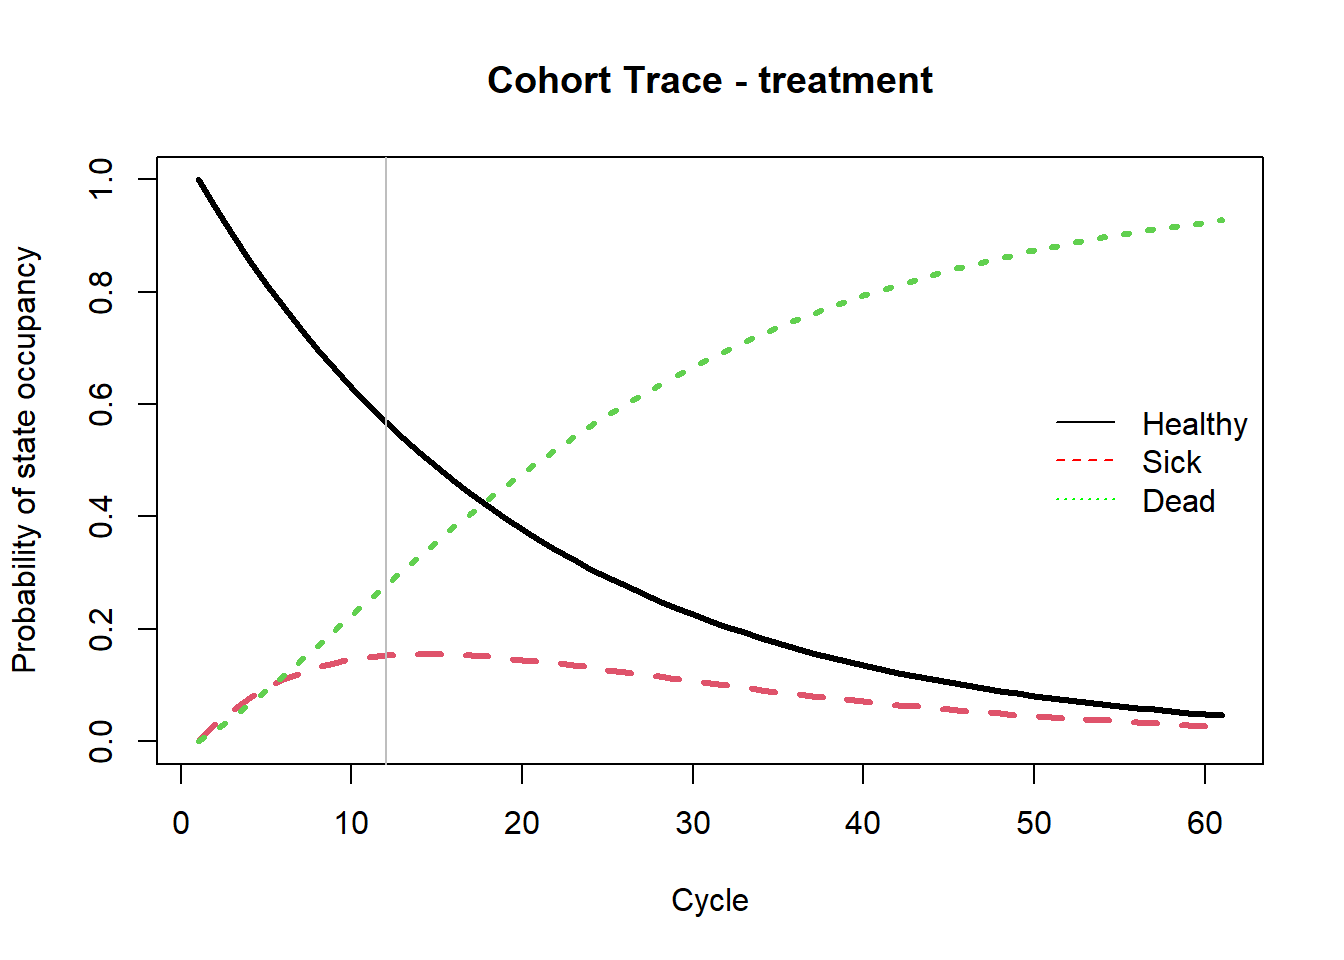
\includegraphics{microsim_3-state_time_files/figure-latex/unnamed-chunk-11-1.pdf}

\begin{Shaded}
\begin{Highlighting}[]
\KeywordTok{plot}\NormalTok{(}\KeywordTok{density}\NormalTok{(outcomes}\OperatorTok{$}\NormalTok{te), }\DataTypeTok{main =} \KeywordTok{paste}\NormalTok{(}\StringTok{"Total QALYs per person"}\NormalTok{), }\DataTypeTok{xlab =} \StringTok{"QALYs"}\NormalTok{)}
\end{Highlighting}
\end{Shaded}

\includegraphics{microsim_3-state_time_files/figure-latex/unnamed-chunk-11-2.pdf}

\begin{Shaded}
\begin{Highlighting}[]
\KeywordTok{plot_m_TR}\NormalTok{(outcomes}\OperatorTok{$}\NormalTok{m_M)    }\CommentTok{# health state trace, function from the "Function.R"-file}
\end{Highlighting}
\end{Shaded}

\includegraphics{microsim_3-state_time_files/figure-latex/unnamed-chunk-11-3.pdf}

\end{document}
